\subsection{Design of the Motor Loop Controller}\label{sec:MotorLoop}

The very first loop control is the one adjusting the motor velocity, $\omega_m$, according to the voltage. The transfer function from $U_m$ to $\omega_{m}$ is taken from \autoref{sec:ModelDCMotor}. \autoref{eq:DCModelNoL} is used with the values for each of its variables: 
\begin{flalign}
\frac{\Omega_m(s)}{U_m(s)}=\frac{0.0293}{3.633\text{e}^{-5}s+0.03138} 
\end{flalign} 

The transfer function has a negative pole making the system stable. A P-controller is enough to control this loop. As it is the most inner loop of the system, the step response has to be faster than the outer loops controlling the arm and the stick. The root locus of the motor loop is plotted next to its step response. 

\begin{figure}[htbp]
	\centering
	\begin{subfigure}{0.48\textwidth}
		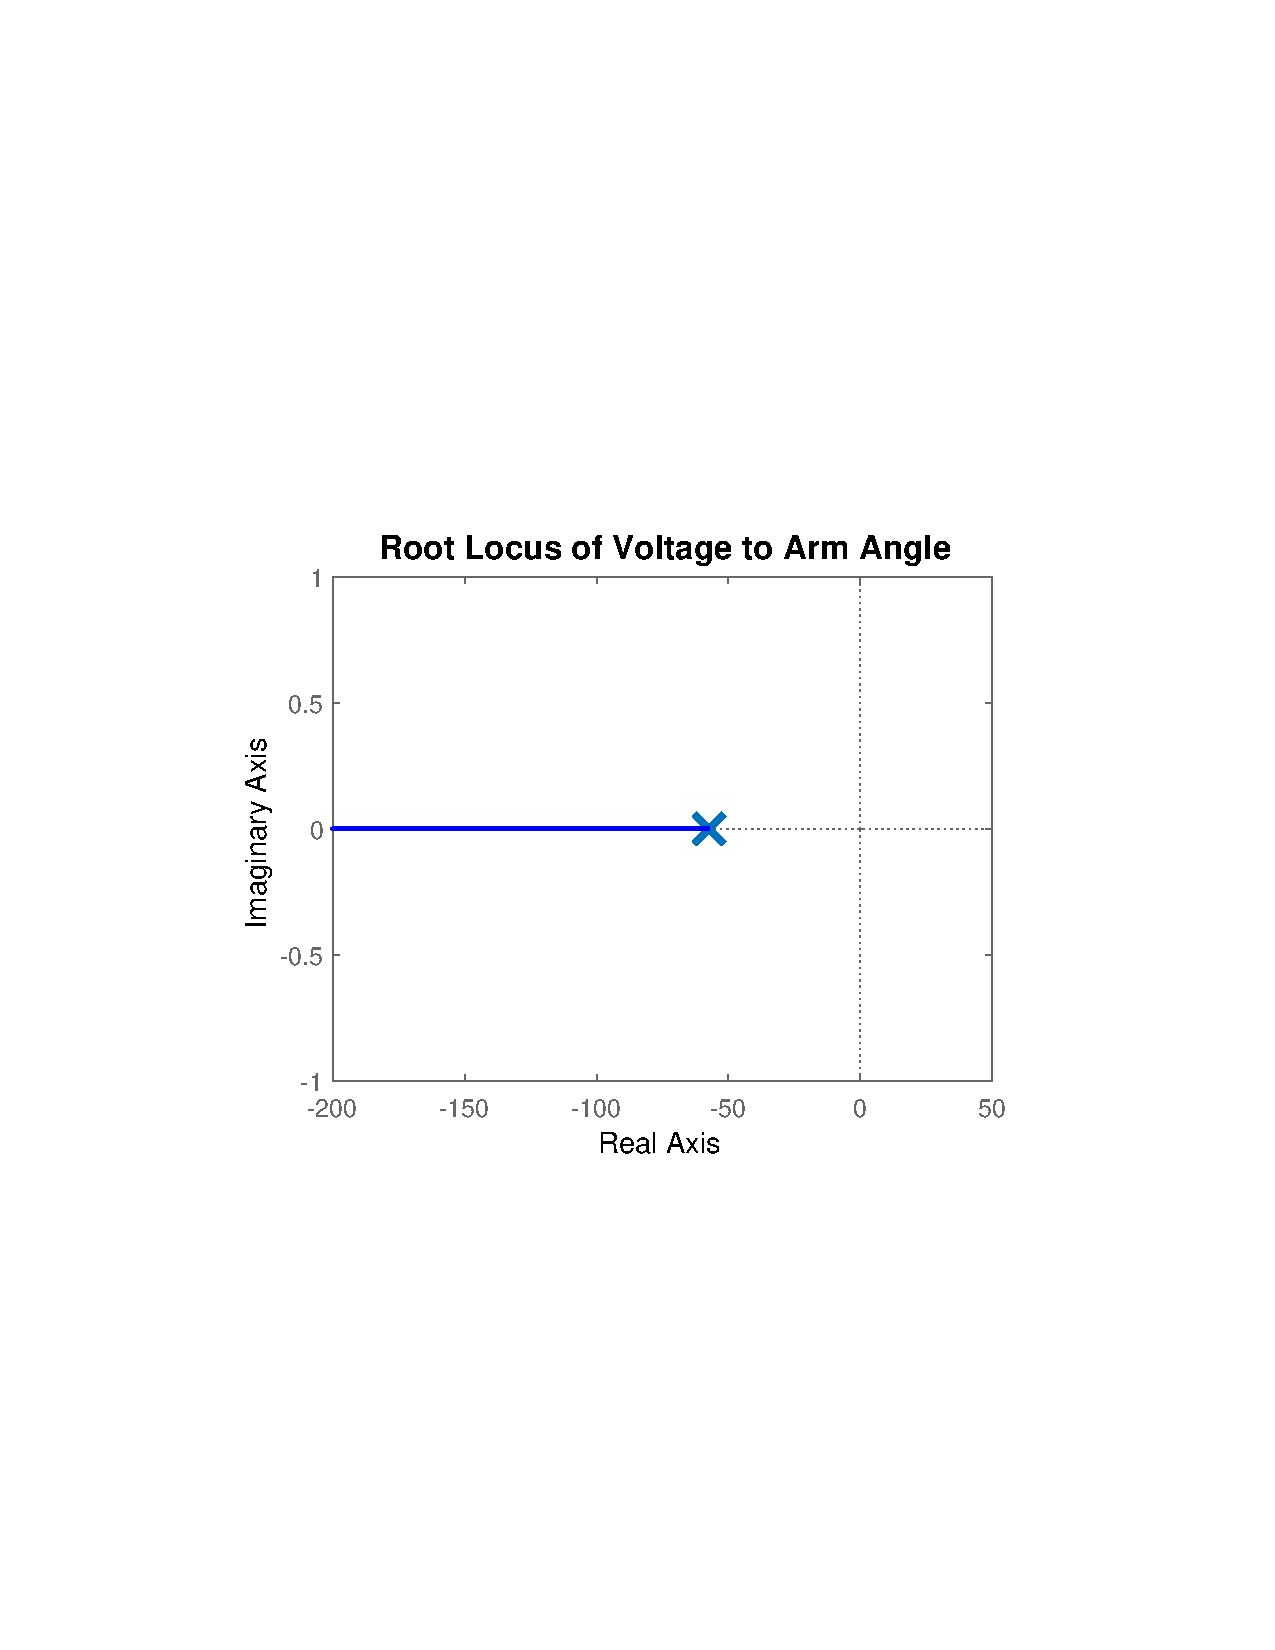
\includegraphics[width=\textwidth]{figures/Design/MotorLoop/MotorRootLocus}
		\caption{Root locus of the motor transfer function}
		\label{fig:MotorRootLocus}
	\end{subfigure}
	\begin{subfigure}{0.5\textwidth}
		\centering
		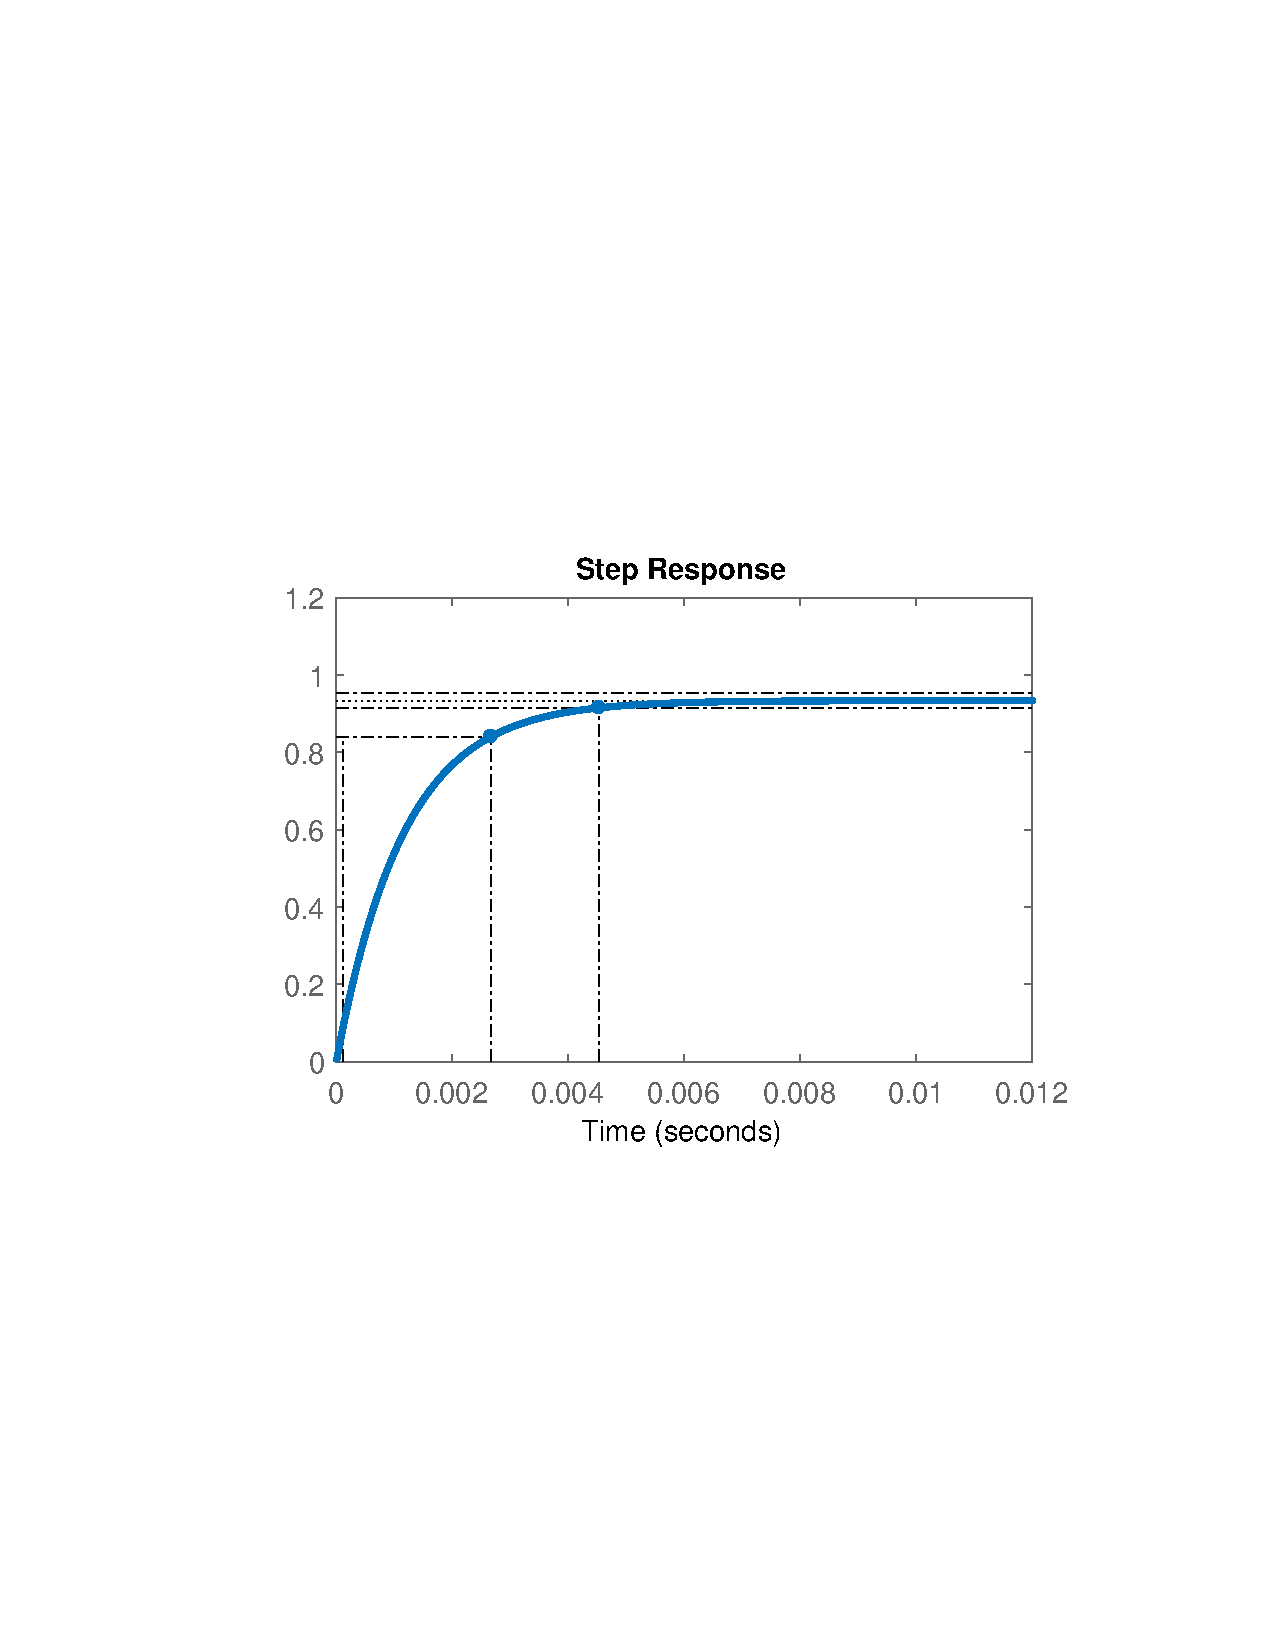
\includegraphics[width=\textwidth]{figures/Design/MotorLoop/MotorStepUncontrolled}
		\caption{Step response of the uncontrolled close loop transfer function}
		\label{fig:fig:MotorStepUncontrolled}
	\end{subfigure}
	\caption{Root locus and step response of the motor loop}
\end{figure}

\autoref{fig:MotorRootLocus} confirms that the motor loop is naturally stable. However, there is a steady state error. The system is then controlled by a P-controller with a gain of 10. 
\begin{figure} [htbp]
	%\hspace*{-3.5cm}
	\centering
	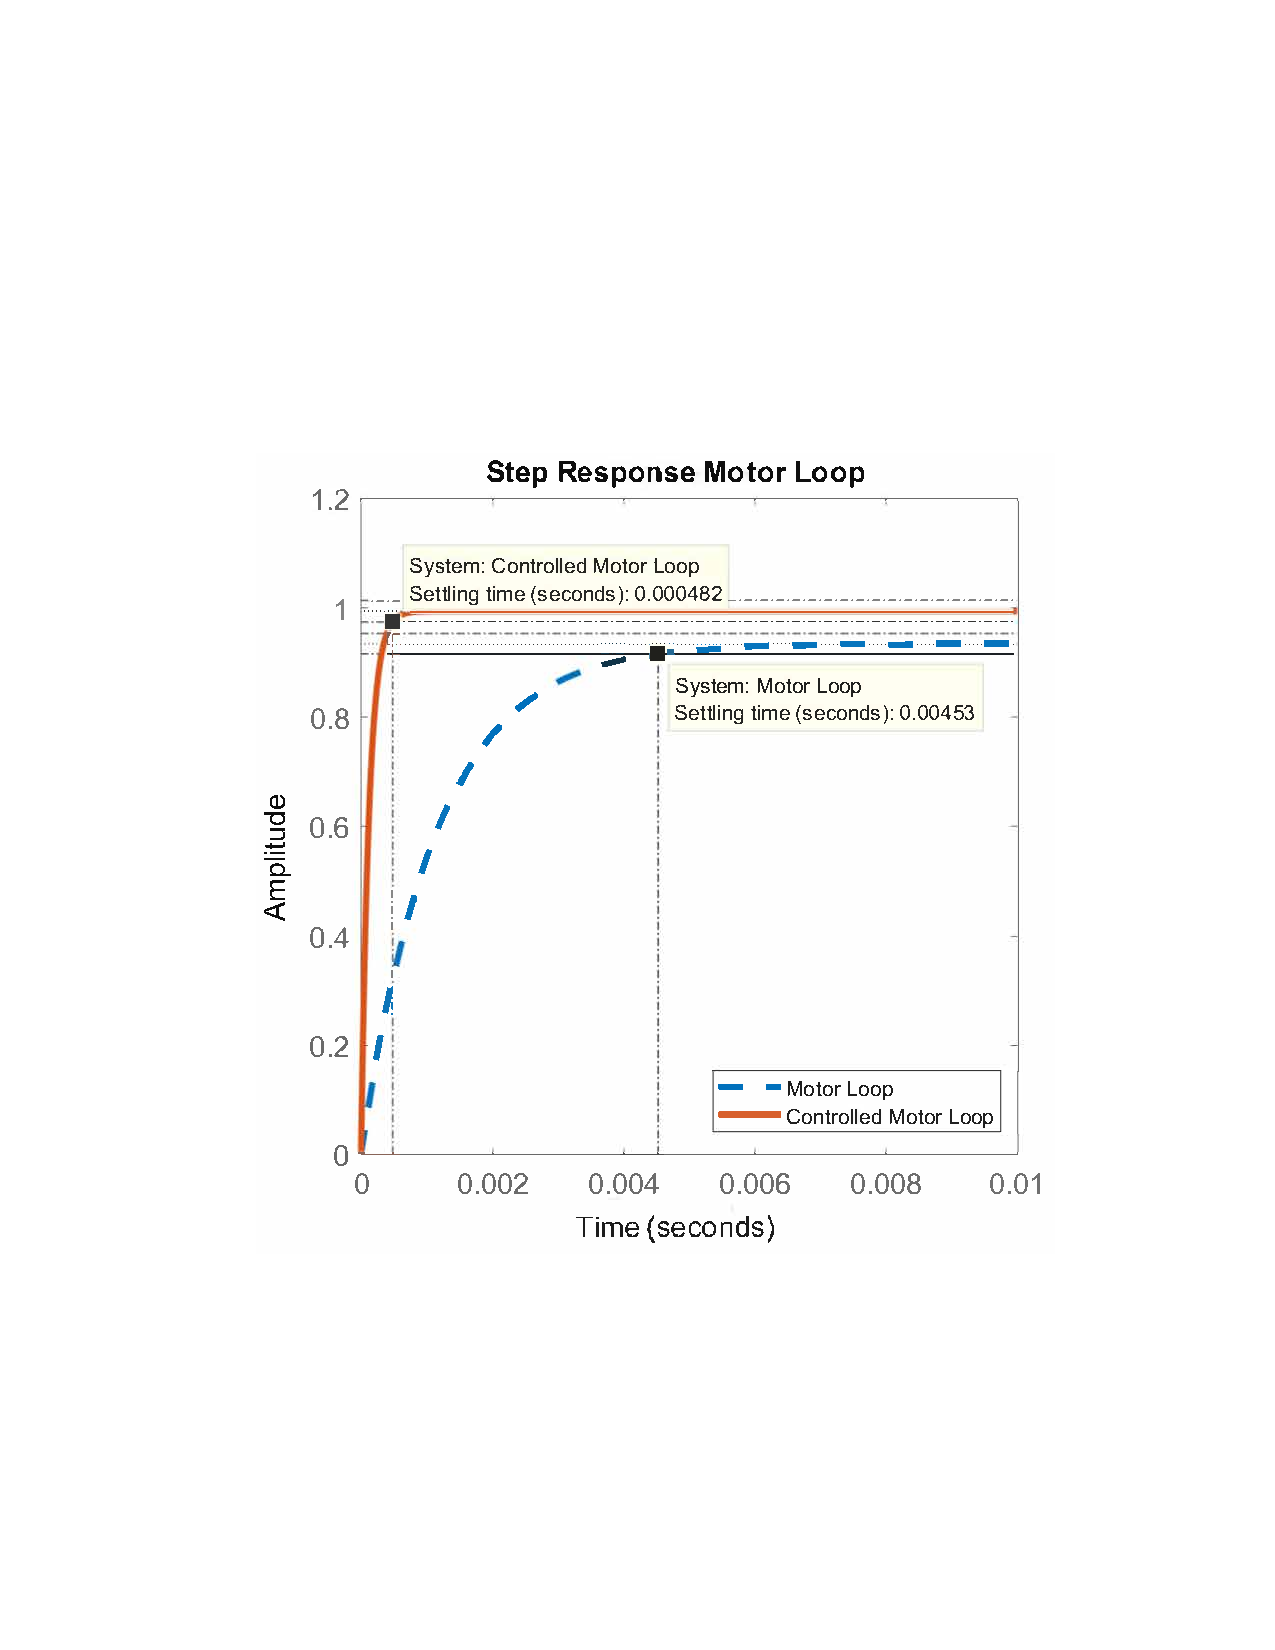
\includegraphics[width=0.7\textwidth]{figures/Design/MotorLoop/MotorStepControlled}
	\caption{Step response of the controlled motor loop.}
	\label{fig:MotorStepControlled}
\end{figure}

As seen on \autoref{fig:MotorStepControlled}, the controlled loop has a rise time of $2.7\text{e}^{-4}$ seconds, ten times faster than the uncontrolled loop. Moreover, the steady state error has decreased from 7\% to 0.01\%. With a proportional gain of 10, the pole is moved far in the left half plane making the motor loop fast enough to be considered as a wire for the arm.

